
\section*{Тренировочное задание, вариант 3}

Осуществить планирование проекта со следующими временными характеристиками:

\begin{figure}[h!]
	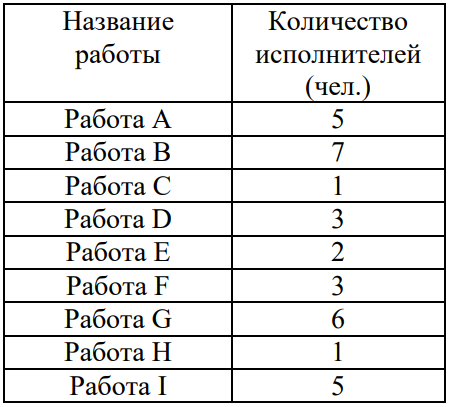
\includegraphics[scale=0.8, center]{train}
\end{figure}

\begin{enumerate}
	\item Дополнить временной план проекта, подготовленный на предыдущем этапе (лабораторная работа № 1), информацией о ресурсах и определить стоимость проекта.
	\item Для этого заполнить ресурсный лист в программе MS Project, принимая во внимание, что к реализации проекта привлекается не более 10 исполнителей..
	\item Предусмотреть, что стандартная ставка ресурс составляет 200 руб./день.
	\item Произвести назначение ресурсов на задачи в соответствии с таблицей. С учетом того, что квалификация ресурсов одинаковая, при назначении ресурсов использовать процент загрузки.
	\item Для выполнения работ С и Е предусмотреть назначение материального ресурса стоимость 100 рублей за штуку и расходом 2 штуки для работы С и 5 штук для работы Е.
\end{enumerate}

Результат: 

\begin{figure}[h!]
	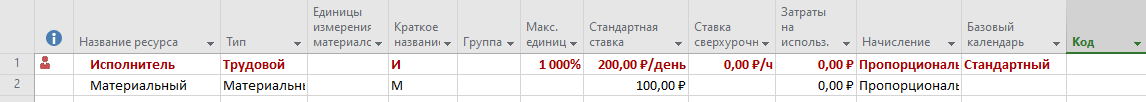
\includegraphics[scale=0.3, center]{train-result-1}
\end{figure}

\begin{figure}[h!]
	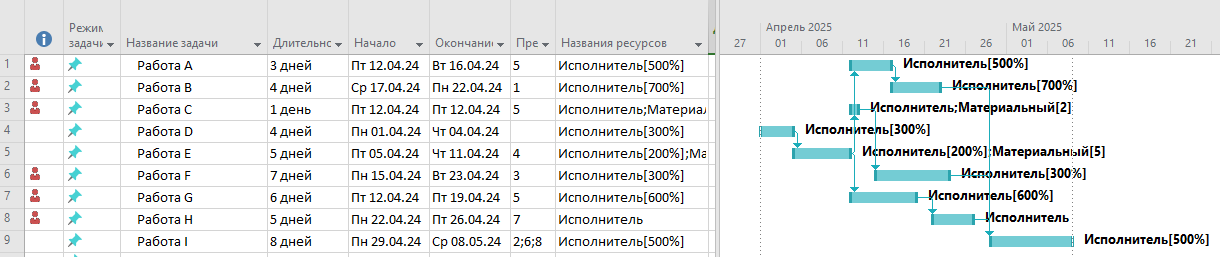
\includegraphics[scale=0.3, center]{train-result-2}
\end{figure}

Видно, что исполнители перегружены и на некоторые задачи не хватает исполнителей.

\clearpage
\section*{Практическое задание}

Целью лабораторной работы №1 является обучение работе с ресурсами в проекте, созданном в Microsoft Project.

\textbf{Содержание проекта:} команда разработчиков из 16 человек занимается созданием карты города на основе собственного модуля отображения. Проект должен быть завершен в течение 6 месяцев. Бюджет проекта: 50 000 рублей.


\subsection*{Задание 1}

Был заполнен ресурсный лист в соответствии с заданием.

\begin{figure}[h!]
	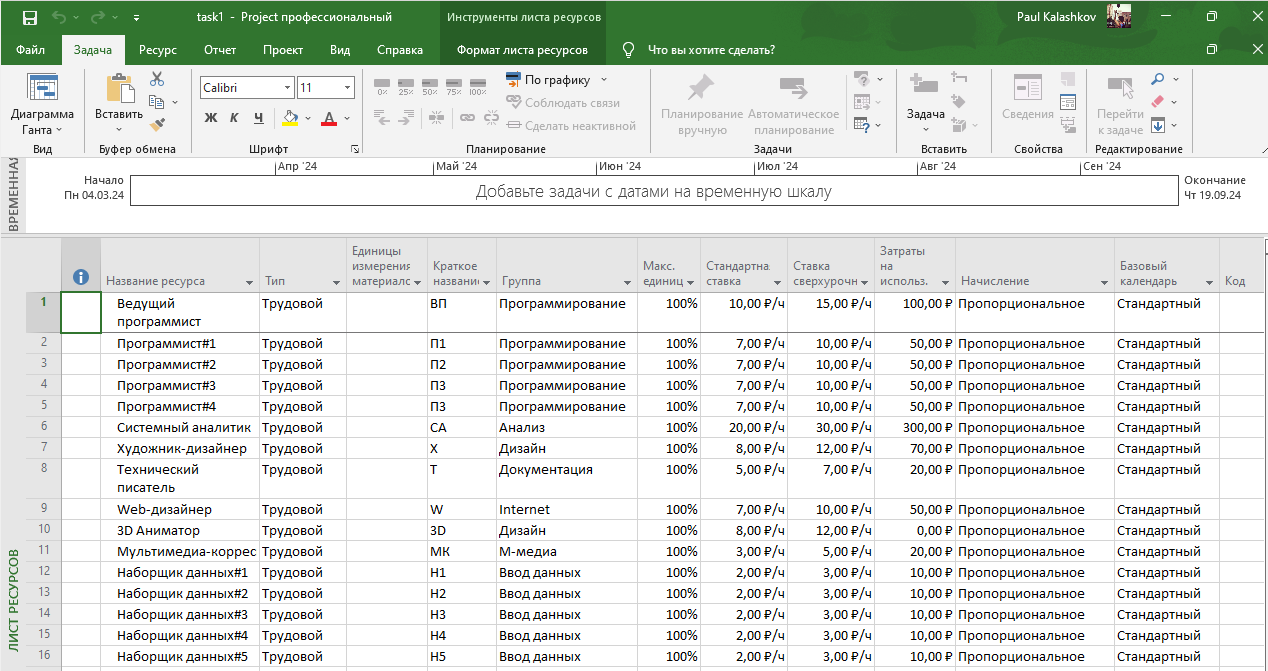
\includegraphics[scale=0.4, center]{task1}
\end{figure}

\subsection*{Задание 2}

Были назначены ресурсы в соответствии с таблицей. 
Исходя из полученных результатов, возникли перегрузки ресурсов, а именно для художника-дизайнера и технического  писателя.

\begin{figure}[h!]
	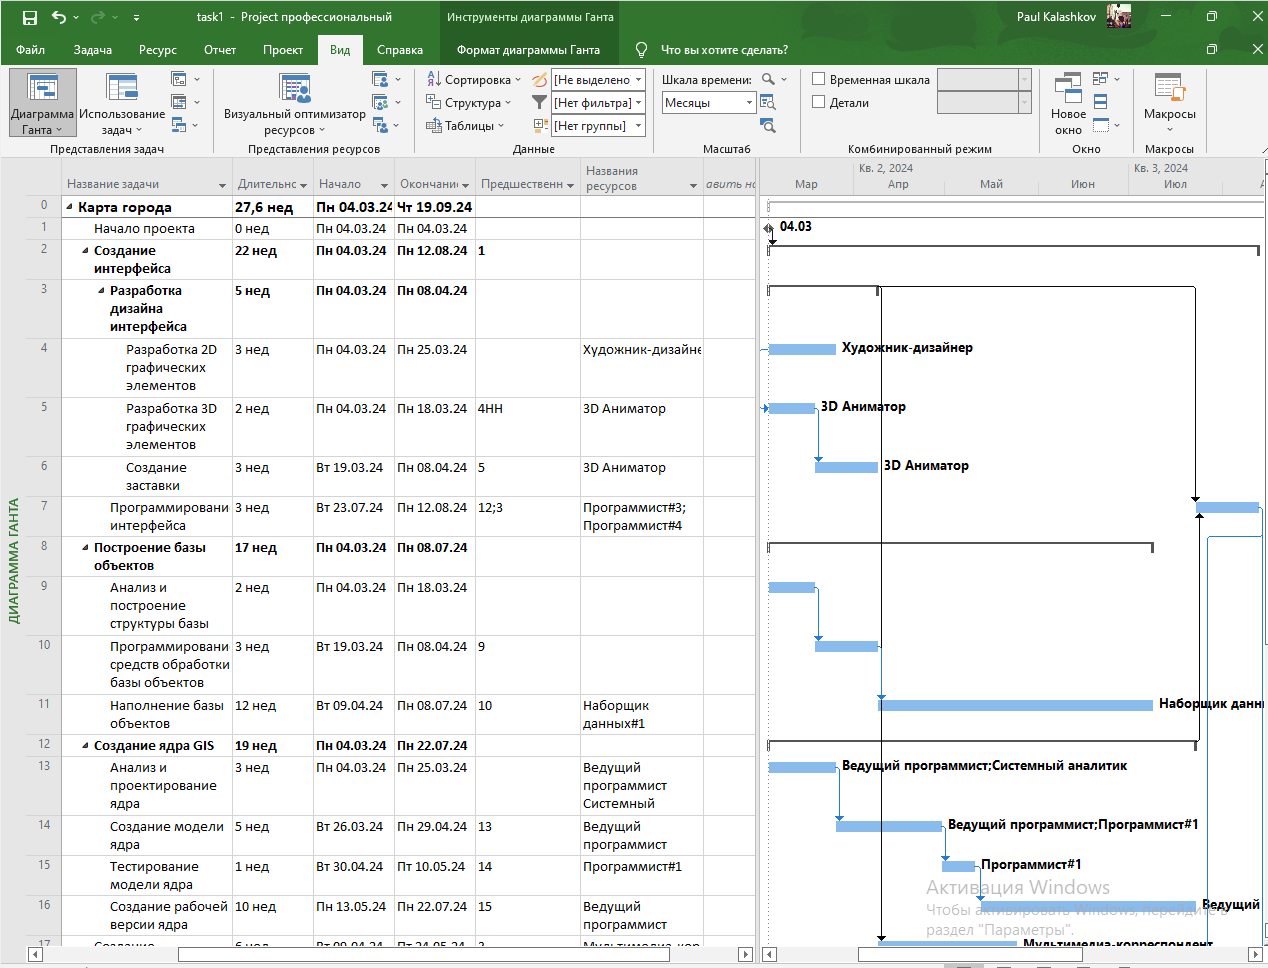
\includegraphics[scale=0.4, center]{task2_1}
\end{figure}

\begin{figure}[h!]
	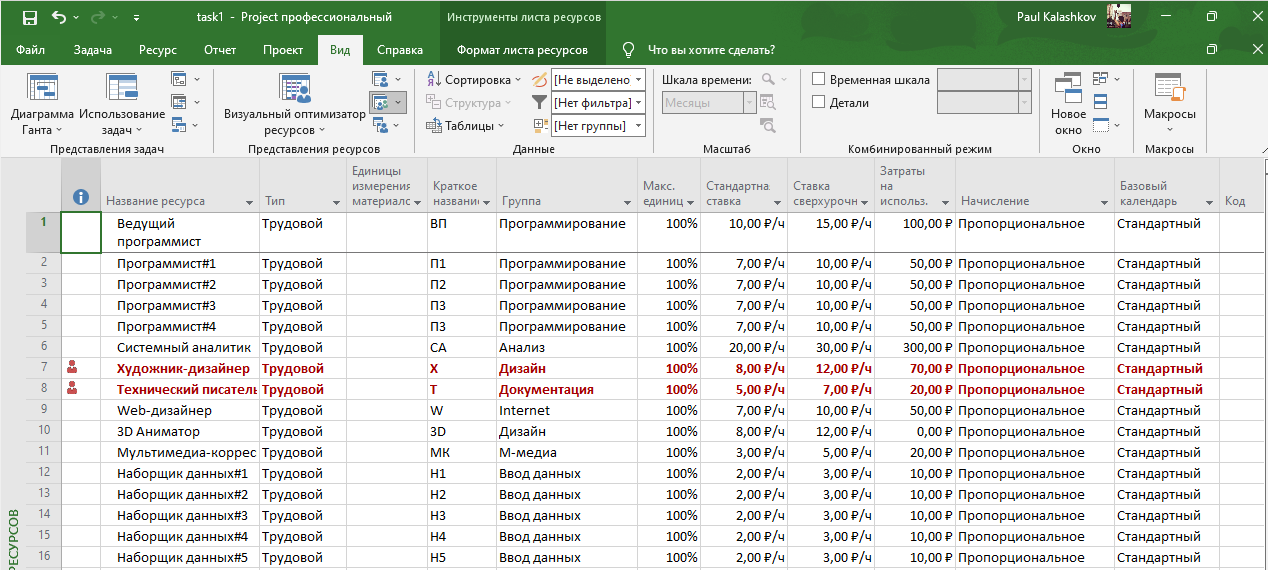
\includegraphics[scale=0.4, center]{task2_2}
\end{figure}
\clearpage

Продемонстрируем это при помощи оптимизатора ресурсов:

\begin{figure}[h!]
	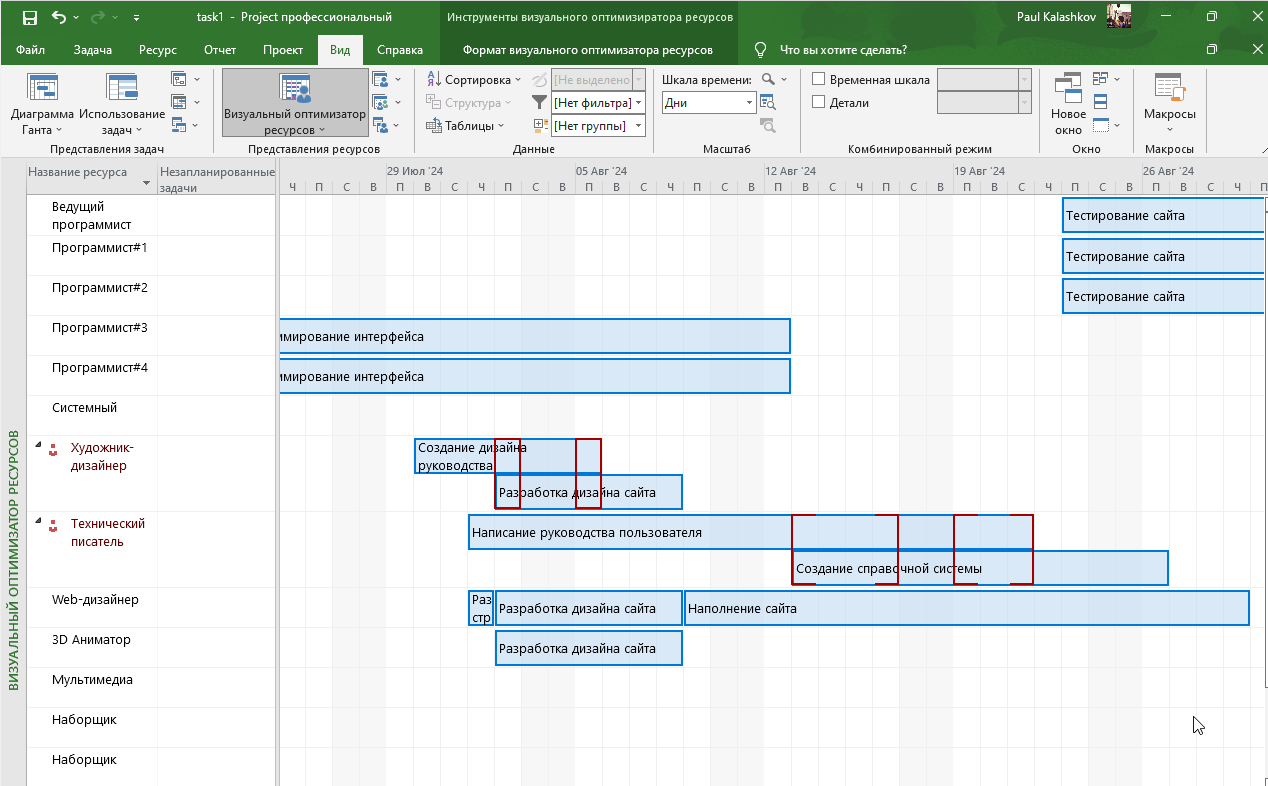
\includegraphics[scale=0.4, center]{task2_3}
\end{figure}

Задачам 2, 8 и 12 были присвоены фиксированные затраты 1000 р.

\begin{figure}[h!]
	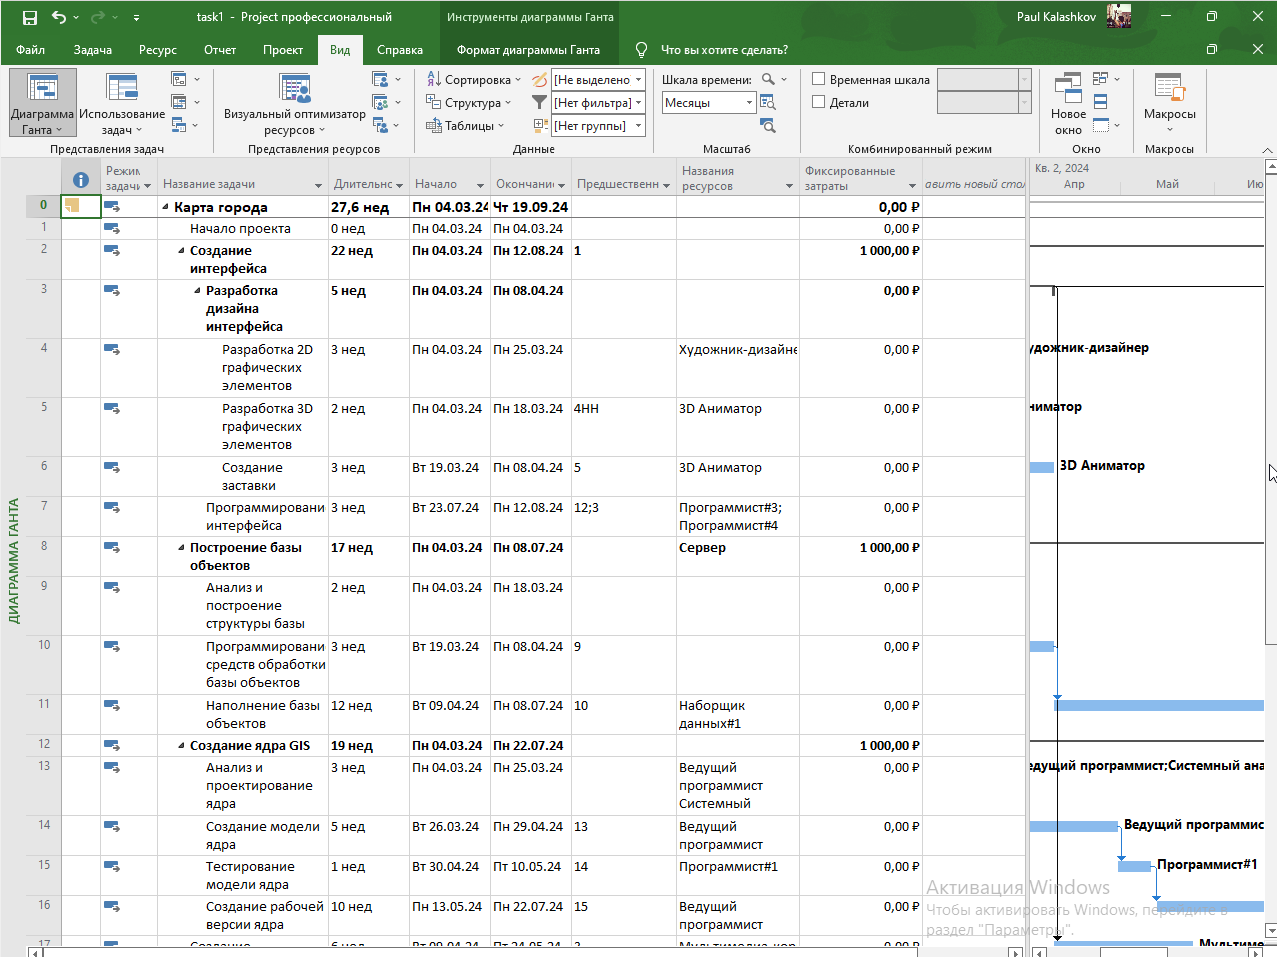
\includegraphics[scale=0.3, center]{task2_4}
\end{figure}

Для задачи 8 был арендован дополнительный сервер (2 рубля за час).
\clearpage
\begin{figure}[h!]
	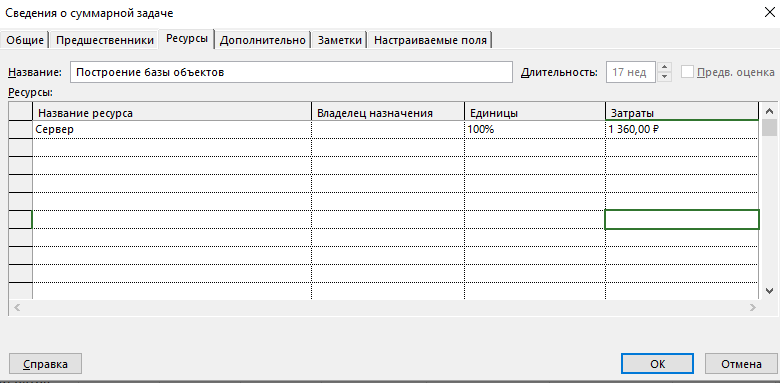
\includegraphics[scale=0.4, center]{task2_5}
\end{figure}

\subsection*{Задание 3}

Было получено использование ресурсов с группировкой по группам.
\begin{figure}[h!]
	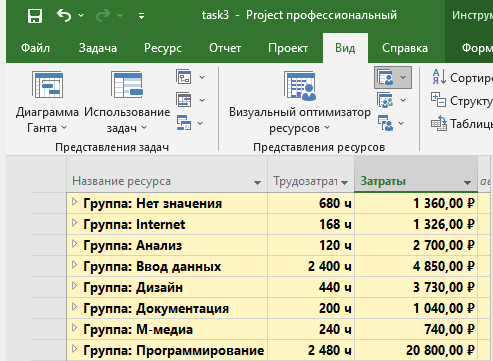
\includegraphics[scale=0.4, center]{task3_1}
\end{figure}

Были построены диаграммы для расчёта процентного соотношения затрат и трудозатрат.

\begin{figure}[h!]
	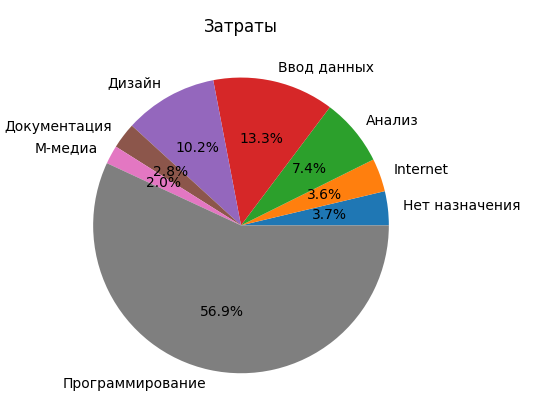
\includegraphics[scale=0.6, center]{task3_2}
\end{figure}

\begin{figure}[h!]
	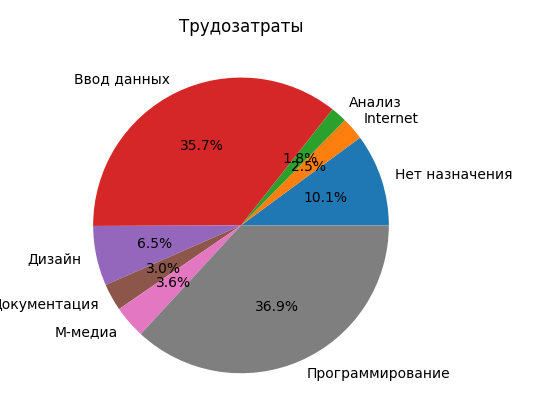
\includegraphics[scale=0.6, center]{task3_3}
\end{figure}


\clearpage

\section*{Заключение}

В ходе выполнения данной лабораторной работы была изучена работа с ресурсами в программе MS Project 2016. Для проекта были определены и поставлены в соответствие с задачами ресурсы (сотрудники, а также дополнительный сервер). 

В результаты затраты по проекту равны 36 546 рублей (укладывается в бюджет). 
Было выявлено, что художник-дизайнер и технический писатель выполняют несколько задач одновременно, то есть происходит перегрузка ресурсов. 
Программисты, выполняя 36.9 процентов работы, занимают 56.9 процентов общего бюджета, в то время как аналитик, выполняя меньше 2 процентов работы, занимает 7.4 процента бюджета.
Требуется оптимизация ресурсов.